\chapter{Future Work}

With this work in hand we did a basic but not fully feature complete implementation of CCH in Neo4j.

There are a lot of specific topics one investigate and implement to improve CCH for Neo4j.

\section{Contraction Algorithms}

Since the contraction Algorithm \ref{alg:contraction} we used definitely has its limitations as we have seen in the experiment section \ref{sec:contraction_limits}, it is worth to further explore this topic.
One very promising method determine the vertex by recursively looking for minimum balanced separators until they tend to get big and then continue with our algorithm.
Another question we have not even touched is, what happens if we add vertices and arcs.
How can we deal with such updates which are not unusual for databases.

\section{The Test Dataset}

Changing the test domain can also be interesting, too.
Papers like CCH \cite{CCH}, CH \cite{Geisberger_2012} and many more focus on road networks.
It sense for this paper to test if we end up to similar results.
However, one could also try grids as Storandt \cite{storandt2013contraction} or look for other real world domains which can be modeled such that shortest path queries are of major interest.

\section{Perfect Customization and Transition to CH}

\begin{wrapfigure}{r}{0.6\textwidth}
    \centering
    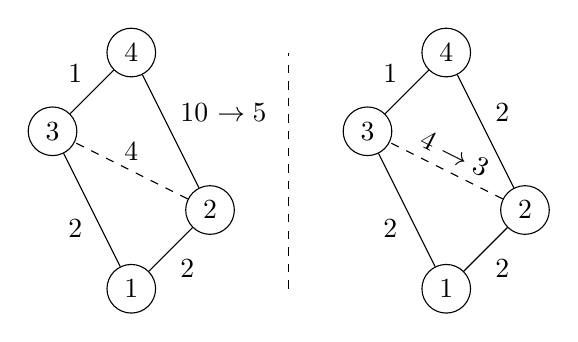
\begin{tikzpicture}[node distance={15mm}, main/.style = {draw, circle}]

    \node[main] (x3) at (0, 2) {$3$};
    \node[main] (x4) at (1, 3) {$4$};
    \node[main] (x2) at (2, 1) {$2$};
    \node[main] (x1) at (1, 0) {$1$};
    
    \draw (x1) -- node[below right] {$2$}(x2);
    \draw (x1) -- node[below left] {$2$} (x3);
    \draw (x2) -- node[above right] {\sout{$10$} $\rightarrow 5$} (x4);
    \draw (x3) -- node[above left] {$1$} (x4);
    \draw[dashed] (x2) -- node[above] {$4$} (x3);

    \draw[dashed]  (3,0) -- (3,3);

    \node[main] (x31) at (4, 2) {$3$};
    \node[main] (x41) at (5, 3) {$4$};
    \node[main] (x21) at (6, 1) {$2$};
    \node[main] (x11) at (5, 0) {$1$};
    
    \draw (x11) -- node[below right] {$2$}(x21);
    \draw (x11) -- node[below left] {$2$} (x31);
    \draw (x21) -- node[above right] {$2$} (x41);
    \draw (x31) -- node[above left] {$1$} (x41);
    \draw[dashed] (x21) -- node[above, sloped] {\sout{$4$} $\rightarrow 3$}  (x31);

    
\end{tikzpicture}
    \caption{Perfect Customization example}
\end{wrapfigure}

Neither did we implement the perfect customization, nor the transition from CCH to CH.
A CH index is usually faster at query time because the amount of arcs to expand is less.
Therefore it can be useful to have a CCH and always calculate a CH from it after each update.
In that scenario it is also useful to measure how the time frame of such.

\section{Using relational Databases}

Furthermore it is questionable if graph databases like Neo4j solve problems.
Due to "The Case Against Specialized Graph Analytics Engines" \cite{fan2015case} there is no significant difference in processing a graph in a graph database compared to a relational database.
Therefore it would be interesting to see how an implementation of dijkstra and (C)CH perform in SQL written for relational databases.
